\documentclass[11pt,a4paper]{article}

% Required packages
\usepackage[utf8]{inputenc}
\usepackage[T1]{fontenc}
\usepackage{graphicx}
\usepackage{subcaption}
\usepackage{amsmath}
\usepackage{amsfonts}
\usepackage{amssymb}
\usepackage{geometry}
\usepackage{float}
\usepackage{booktabs}
\usepackage{array}

% Page setup 
\geometry{margin=2.5cm}
\setlength{\parindent}{0pt}
\setlength{\parskip}{6pt}

% Title and date
\title{Bacterial Signaling Circuit Simulation Update}
\author{} % Add your name here if needed

\begin{document}

\maketitle

% ============================================================================
% MONOTONIC DECREASING CIRCUIT
% ============================================================================
\section{Monotonic Decreasing Circuit}

\subsection{Circuit}

\begin{figure}[H]
    \centering
    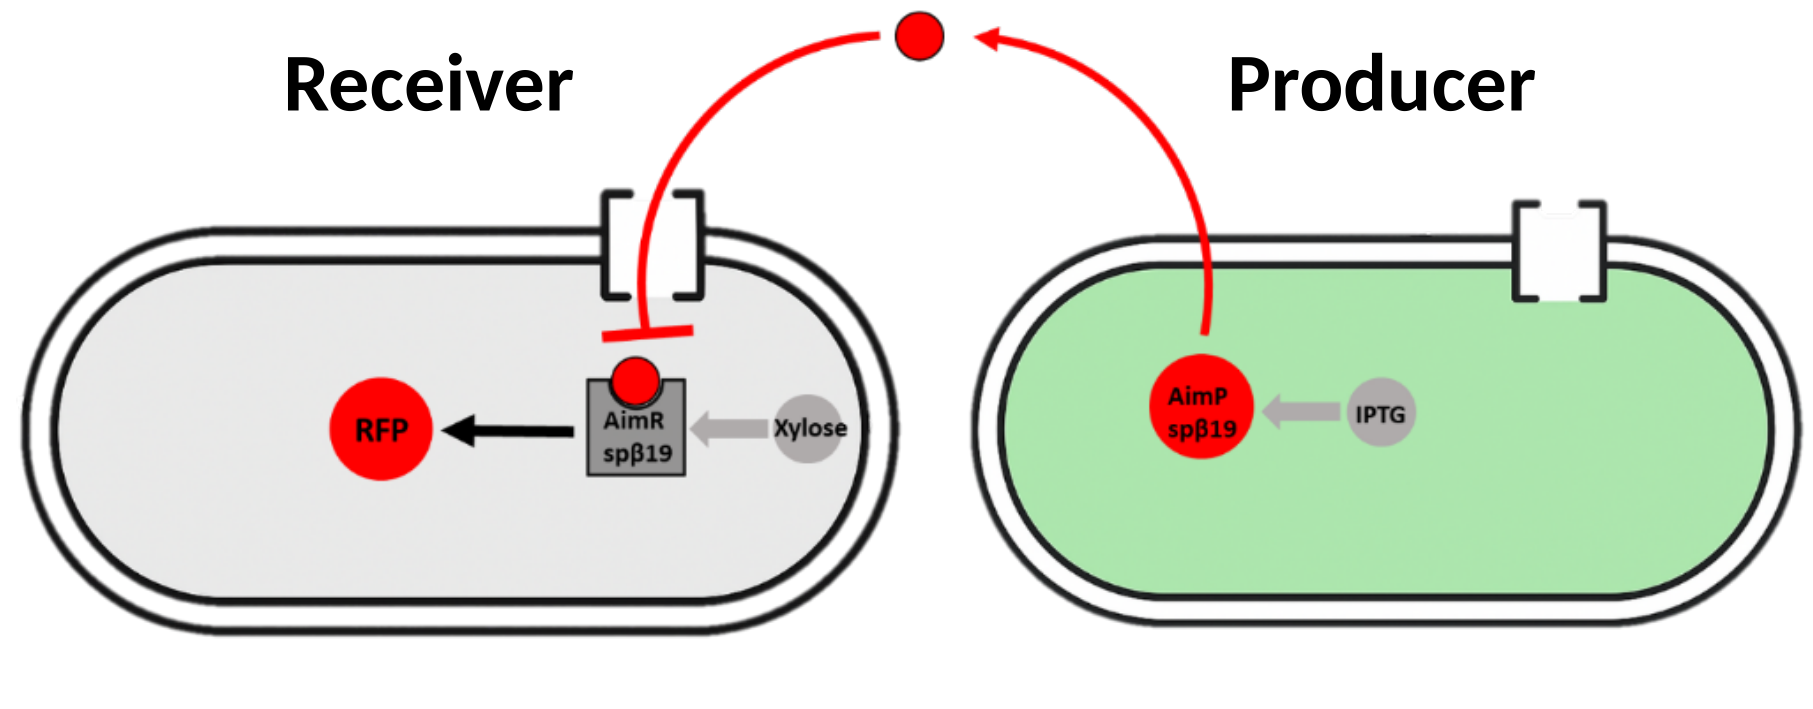
\includegraphics[width=0.8\textwidth]{../figures/diagramMonDec.png}
    \label{fig:mono_dec_schematic}
\end{figure}

\textbf{Intracellular AimP ($P_i$) and AimR ($R_i$) for a receiver bacteria $i$ at a location $r_i$:}
\begin{align*}
\frac{\partial P_i}{\partial t} =& K_{in} P(r_i)^{ext} - K_{on} P_i R_i - \beta P_i\\
\frac{\partial R_i}{\partial t} =& K_{syn} \frac{x}{K_x + x}  - K_{on} P_i R_i - \alpha R_i
\end{align*}

where $x$ is xylose.


\textbf{Intracellular AimP ($P_j$) for a producer bacteria $j$ at a location $r_j$:}
\begin{align*}
\frac{\partial P_j}{\partial t} =& K_{in} P(r_j)^{ext} - \beta P_j\\
\end{align*}

assuming producer bacteria does not contain any AimR in the cytoplasm. This equation is decoupled from all other equations and does not play an important role for this particular circuit.


\textbf{Extracellular AimP concentration:}
\begin{equation}
    \frac{\partial P(r)^{ext}}{\partial t} = K_{out} \frac{I}{K_{I} + I} \sum_{j}^{N} \delta(r_j - r)  - K_{in} \sum_{b}^{N} P(r_b)^{ext}\delta(r_b - r)+ D_p \cdot \nabla^2 P(r)^{ext}
\end{equation}

where $I$ is IPTG, $b$ is any bacteria (producers and receiver), and $r_j$ is the locations of the producer bacteria.

\subsection{Simulation vs. Real-World Comparison}

\begin{figure}[H]
    \centering
    \begin{subfigure}[b]{0.45\textwidth}
        \centering
        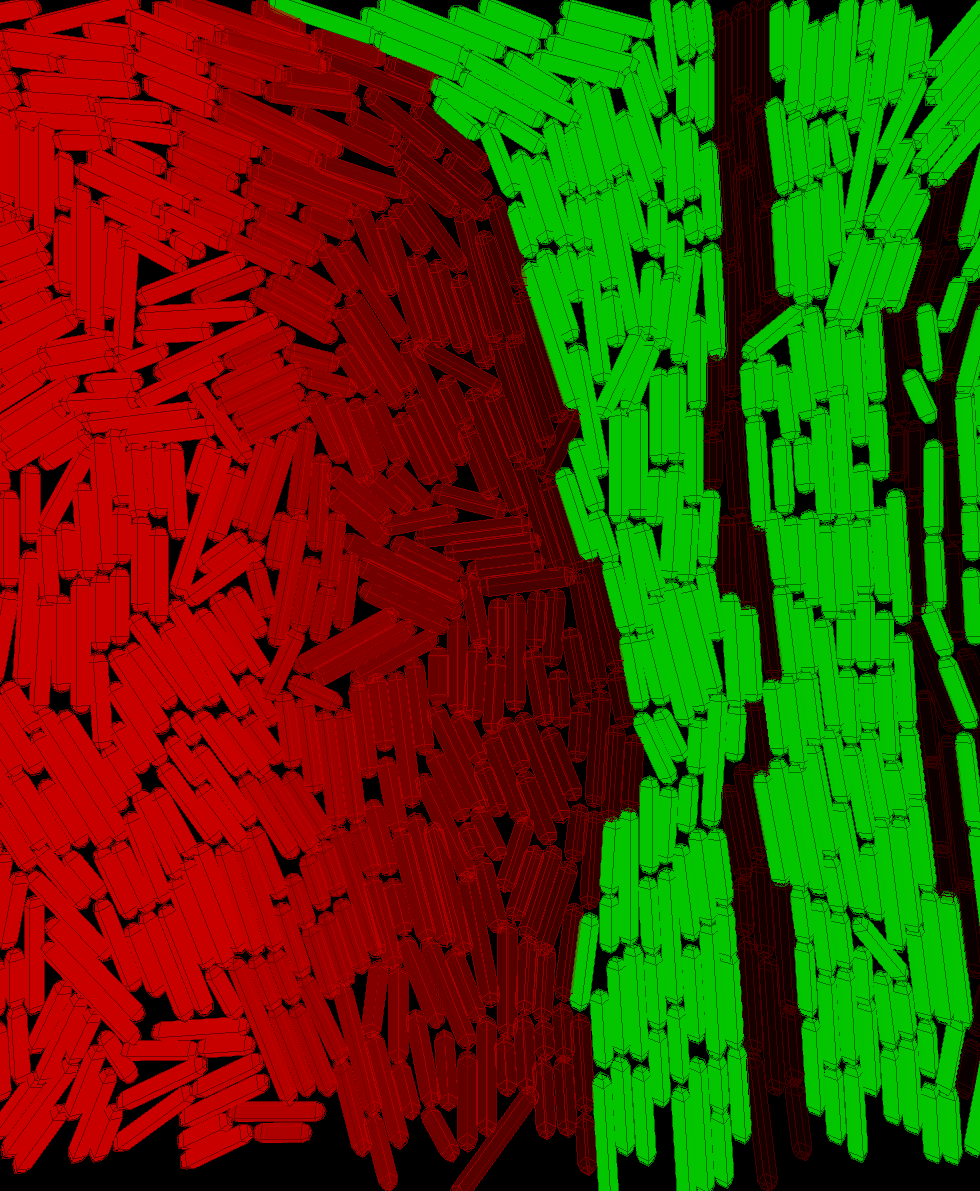
\includegraphics[width=\textwidth]{../figures/monDecSim.png}
        \caption{Simulation Result}
        \label{fig:mono_dec_sim}
    \end{subfigure}
    \hfill
    \begin{subfigure}[b]{0.45\textwidth}
        \centering
        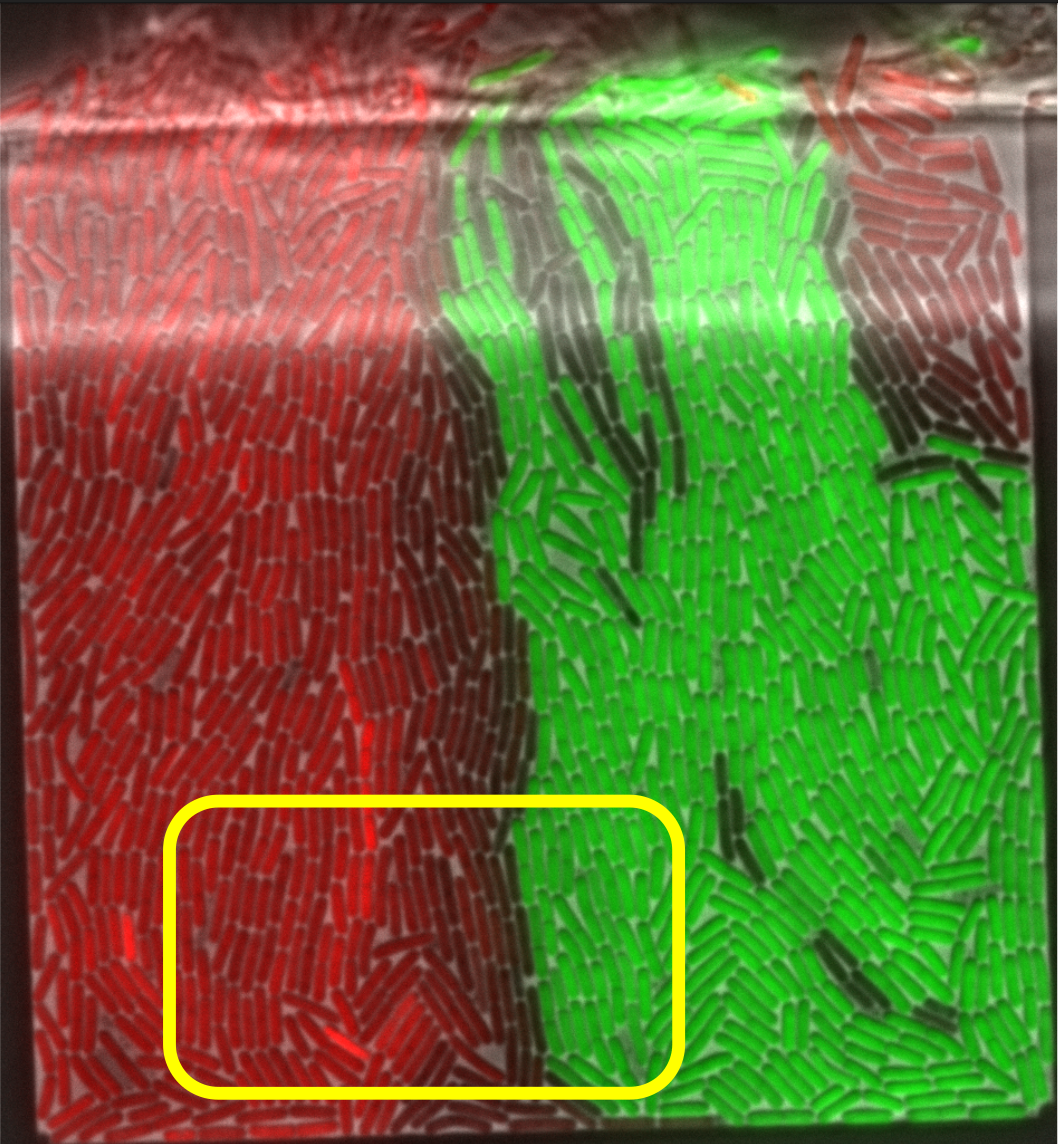
\includegraphics[width=\textwidth]{../figures/monotonicDecreasingReal.png}
        \caption{Microfluidics Chamber}
        \label{fig:mono_dec_real}
    \end{subfigure}
    \label{fig:mono_dec_comparison}
\end{figure}

% ============================================================================
% MONOTONIC INCREASING CIRCUIT
% ============================================================================
\section{Monotonic Increasing Circuit}

\subsection{Circuit}

\begin{figure}[H]
    \centering
    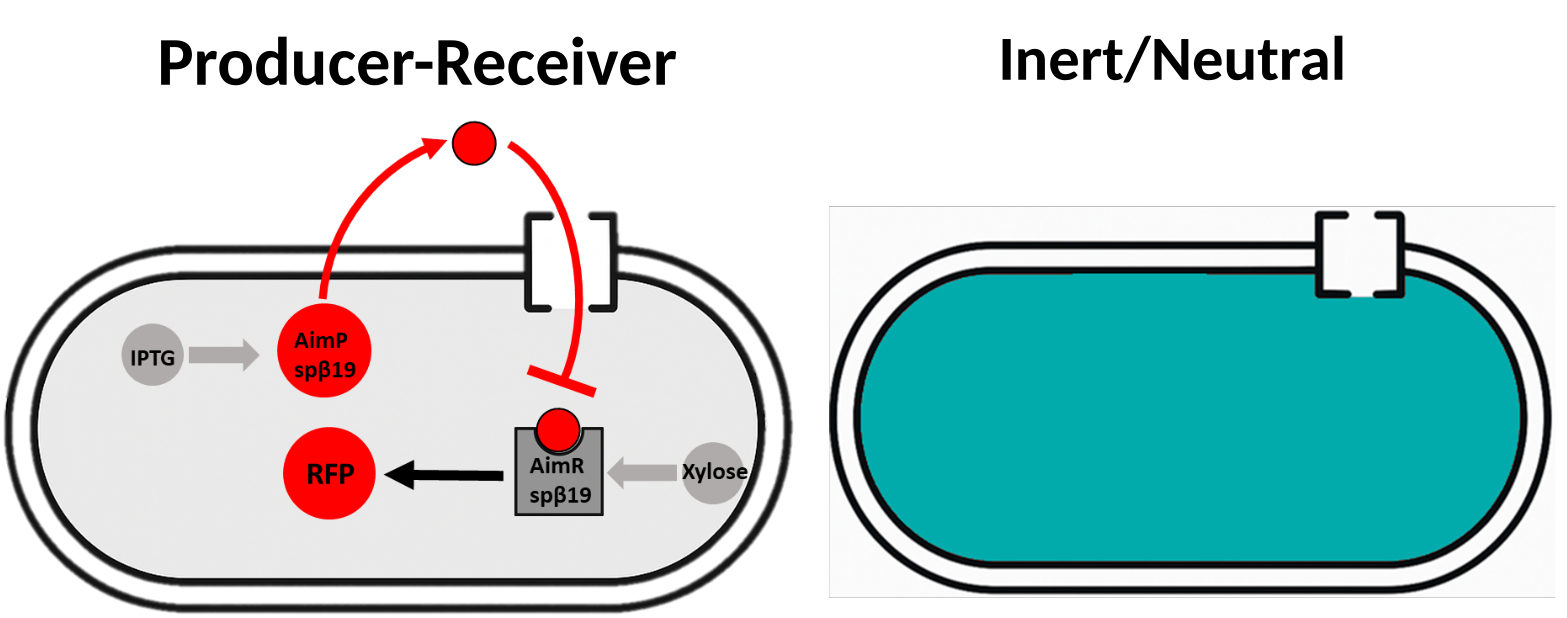
\includegraphics[width=0.8\textwidth]{../figures/monIncDiag.png}
    \label{fig:mono_dec_schematic}
\end{figure}

\textbf{Intracellular AimP ($P_i$) and AimR ($R_i$) for a producer-receiver bacteria $i$ at a location $r_i$:}
\begin{align*}
\frac{\partial P_i}{\partial t} =& K_{in} P(r_i)^{ext} - K_{on} P_i R_i - \beta P_i \\
\frac{\partial R_i}{\partial t} =& K_{syn} \frac{x}{K_x + x} - K_{on} P_i R_i - \alpha R_i 
\end{align*}

\textbf{Intracellular AimP ($P_o$)  for a neutral bacteria $o$ at a location $r_o$:}
\begin{align*}
\frac{\partial P_o}{\partial t} =& K_{in} P(r_o)^{ext}  - \beta P_o \\
\end{align*}
This equation is decoupled from all other equations and does not play an important role for this particular circuit.

\textbf{Extracellular AimP concentration:}
\begin{equation}
    \frac{\partial P(r)^{ext}}{\partial t} = K_{out} \frac{I}{K_{I} + I} \sum_{i}^{N} \delta(r_i - r)  - K_{in} \sum_{b}^{N} P(r_b)^{ext}\delta(r_b - r)+ D_p \cdot \nabla^2 P(r)^{ext}
\end{equation}

where $I$ is IPTG, $i$ are producer-receiver bacteria, $b$ is a bacteria of any phenotype (producers-receiver and neutral), $r_i$ are the locations of the producers-receiver bacteria, and 
$r_b$ are the locations of bacteria of any phenotype (producers-receiver and neutral).

\subsection{Simulation vs. Real-World Comparison}

\begin{figure}[H]
    \centering
    \begin{subfigure}[b]{0.45\textwidth}
        \centering
        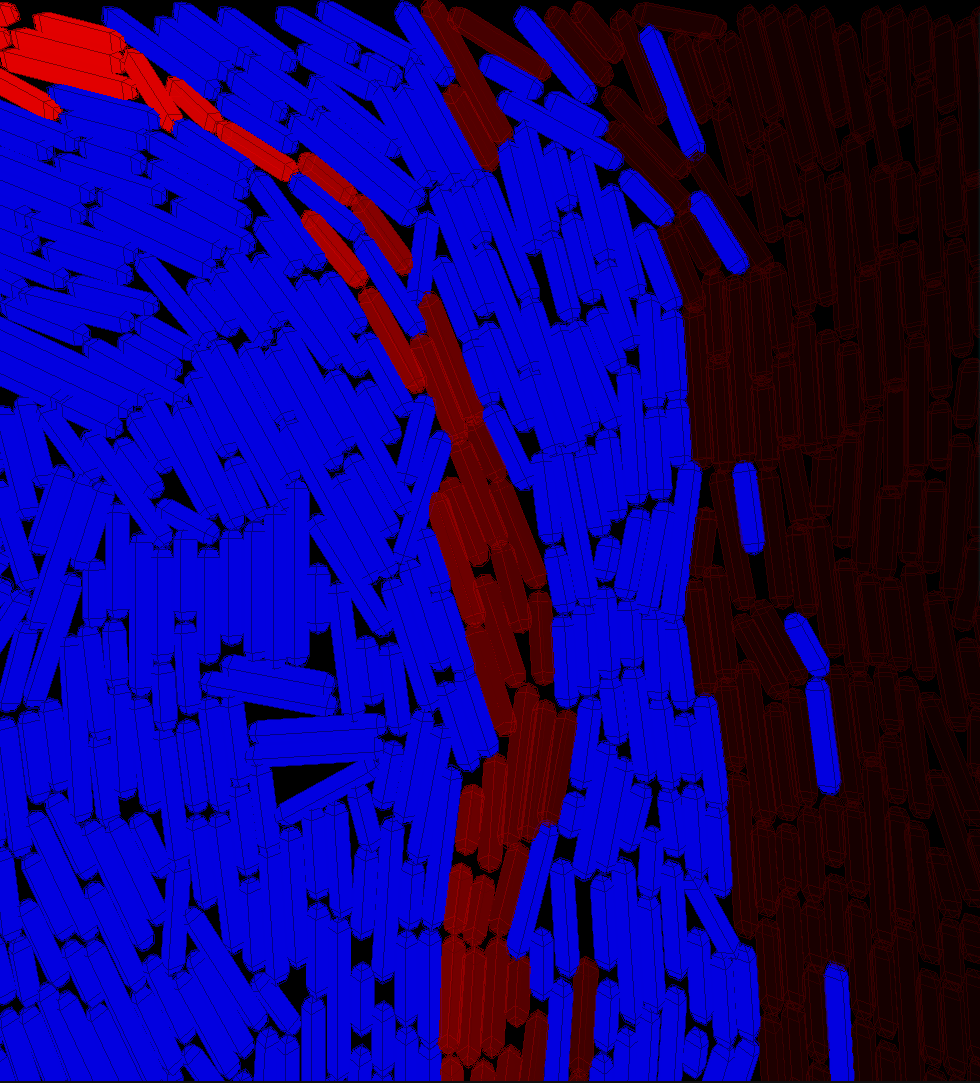
\includegraphics[width=\textwidth]{../figures/monInSim.png}
        \caption{Simulation Result}
        \label{fig:mono_dec_sim}
    \end{subfigure}
    \hfill
    \begin{subfigure}[b]{0.45\textwidth}
        \centering
        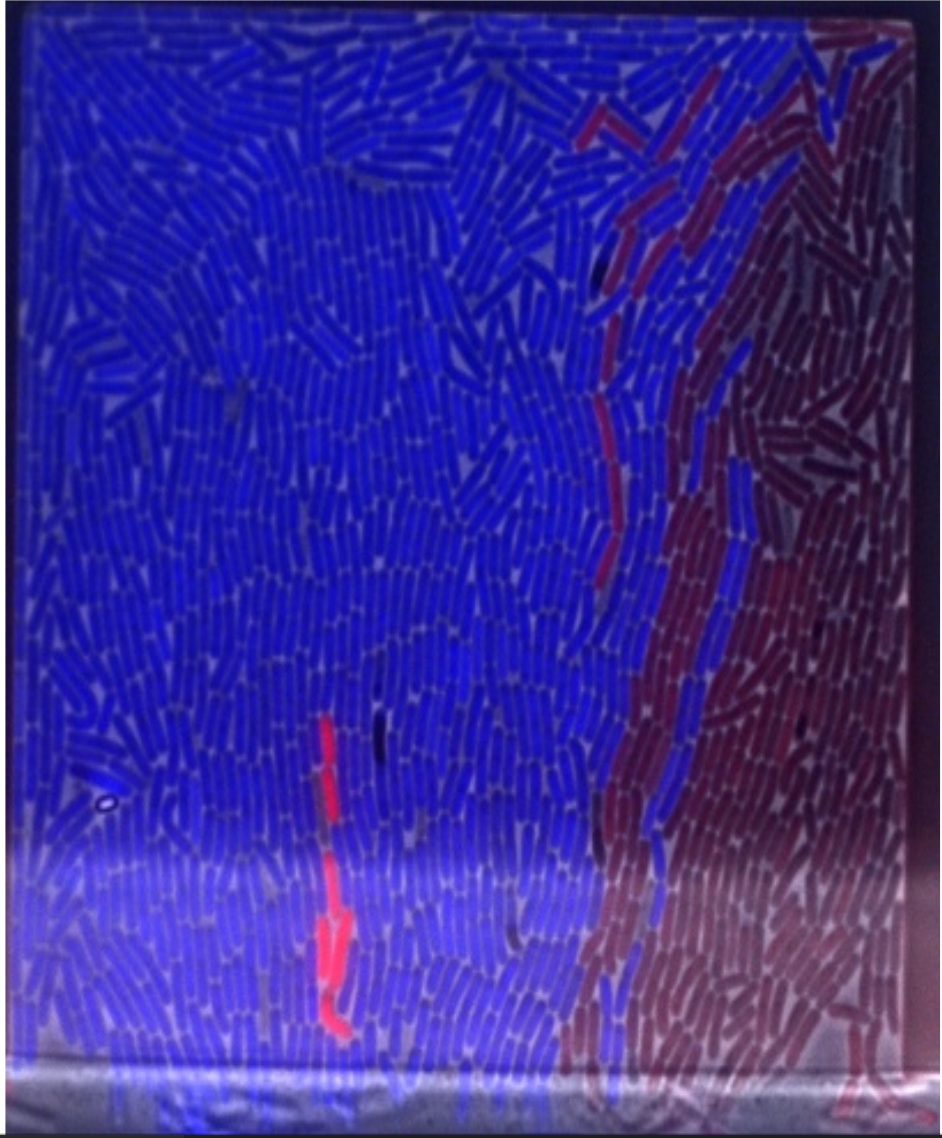
\includegraphics[width=\textwidth]{../figures/MonIncrReal.png}
        \caption{Microfluidics Chamber}
        \label{fig:mono_dec_real}
    \end{subfigure}
    \label{fig:mono_dec_comparison}
\end{figure}

% ============================================================================
%  SWITCHLIKE CIRCUIT
% ============================================================================
\section{Switch-like Circuit}

\subsection{Circuit}

\begin{figure}[H]
    \centering
    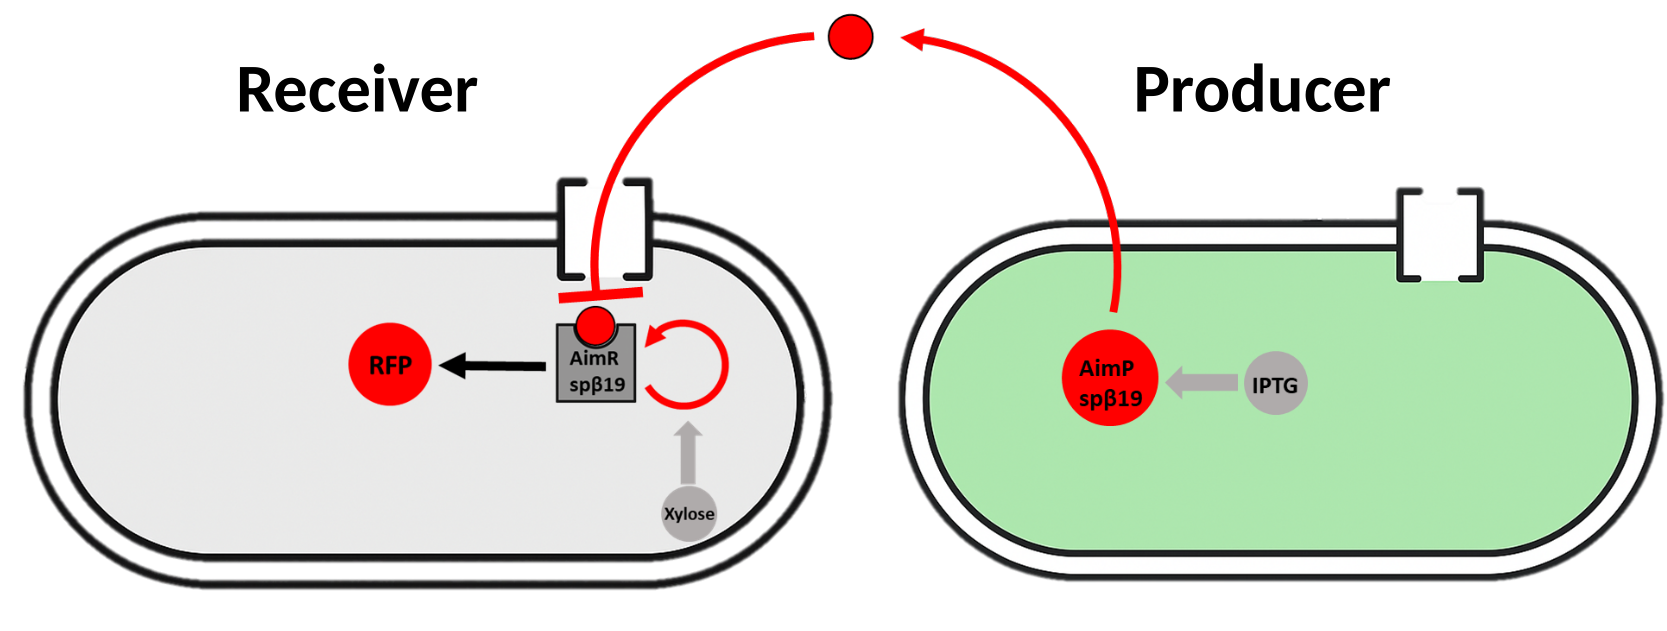
\includegraphics[width=0.8\textwidth]{../figures/SwitchLikeDiag.png}
    \label{fig:mono_dec_schematic}
\end{figure}

\textbf{Intracellular AimP ($P_i$) and AimR ($R_i$) for a receiver bacteria $i$ at a location $r_i$:}
\begin{align*}
\frac{\partial P_i}{\partial t} =& K_{in} P(r_i)^{ext} - K_{on} P_i R_i - \beta P_i\\
\frac{\partial R_i}{\partial t} =& K_b + K_{syn} \frac{x}{K_x + x} \cdot \frac{R_i^n}{K_r^n + R_i^n} - K_{on} P_i R_i - \alpha R_i 
\end{align*}

where $n$ is the Hill coefficient and $K_b$ is the basal production rate of AimR. The basal production rate $K_b$ had to be included in the equation to avoid AimR's concentration reaching values near to zero, which would 
otherwise make it very dificult for the switch to turn on.

\textbf{Intracellular AimP ($P_j$) for a producer bacteria $j$ at a location $r_j$:}
\begin{align*}
\frac{\partial P_j}{\partial t} =& K_{in} P(r_j)^{ext} - \beta P_j\\
\end{align*}

assuming producer bacteria does not contain any AimR in the cytoplasm. This equation is decoupled from all other equations and does not play an important role for this particular circuit.

\textbf{Extracellular AimP concentration:}
\begin{equation}
    \frac{\partial P(r)^{ext}}{\partial t} = K_{out} \frac{I}{K_{I} + I} \sum_{j}^{N} \delta(r_j - r)  - K_{in} \sum_{b}^{N} P(r_b)^{ext}\delta(r_b - r)+ D_p \cdot \nabla^2 P(r)^{ext}
\end{equation}

where $I$ is IPTG, $b$ is any bacteria (producers and receiver), and $r_j$ is the locations of the producer bacteria.

\subsection{Simulation vs. Real-World Comparison}

\begin{figure}[H]
    \centering
    \begin{subfigure}[b]{0.45\textwidth}
        \centering
        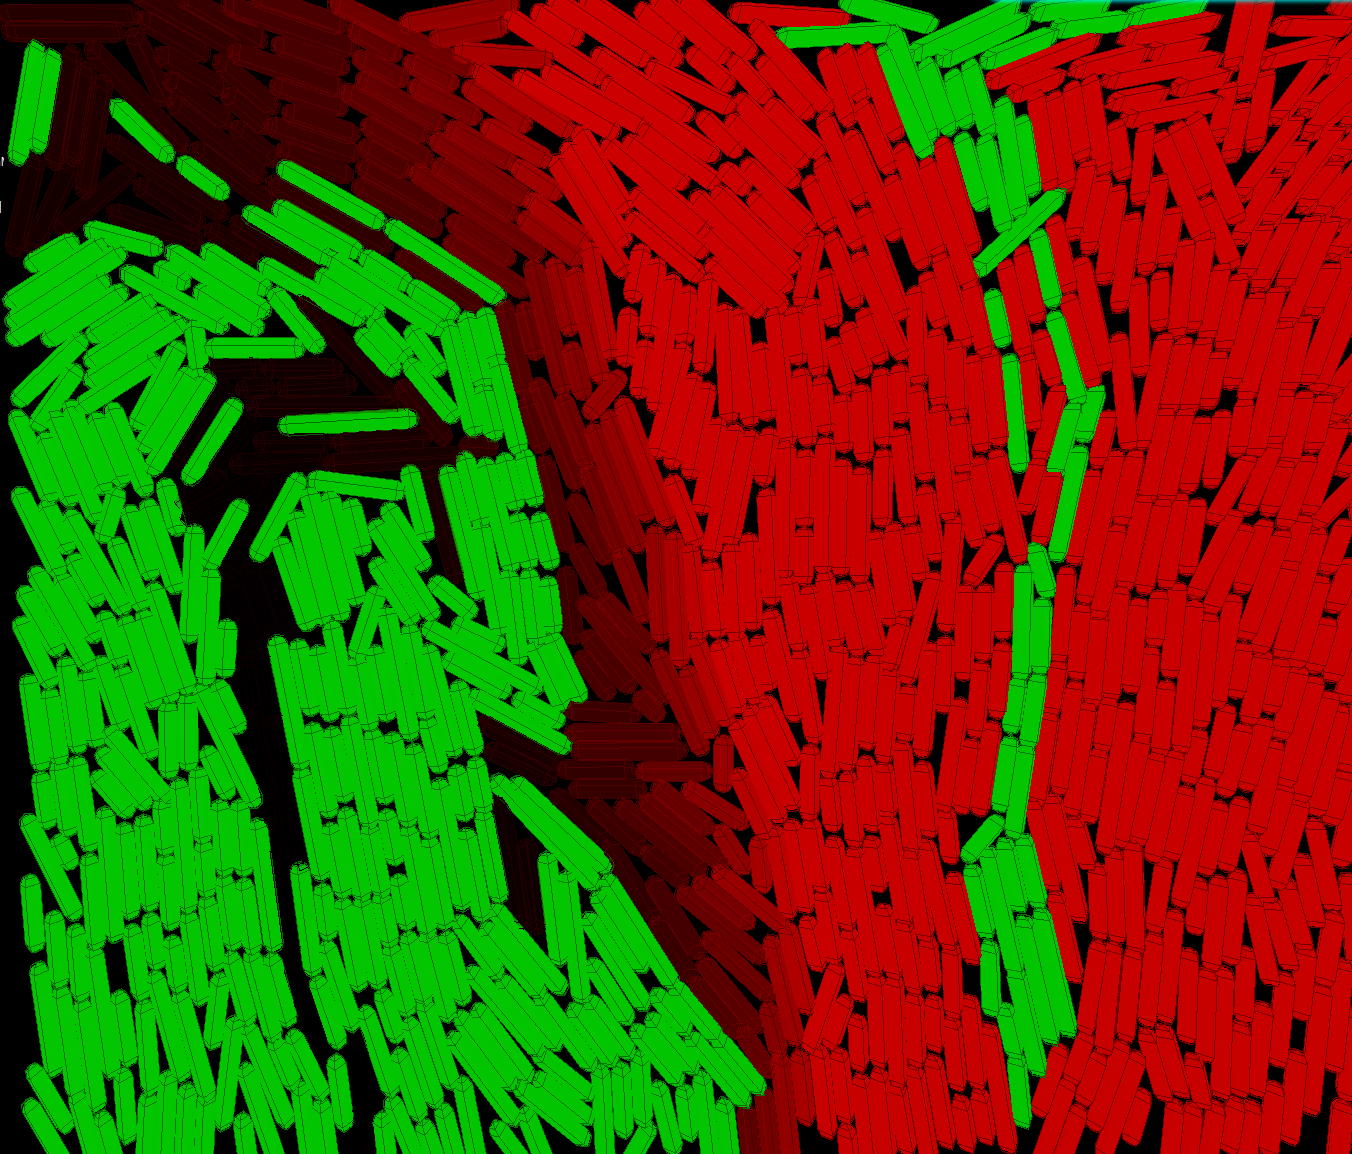
\includegraphics[width=\textwidth]{../figures/switchLikeSim.png}
        \caption{Simulation Result}
        \label{fig:mono_dec_sim}
    \end{subfigure}
    \hfill
    \begin{subfigure}[b]{0.45\textwidth}
        \centering
        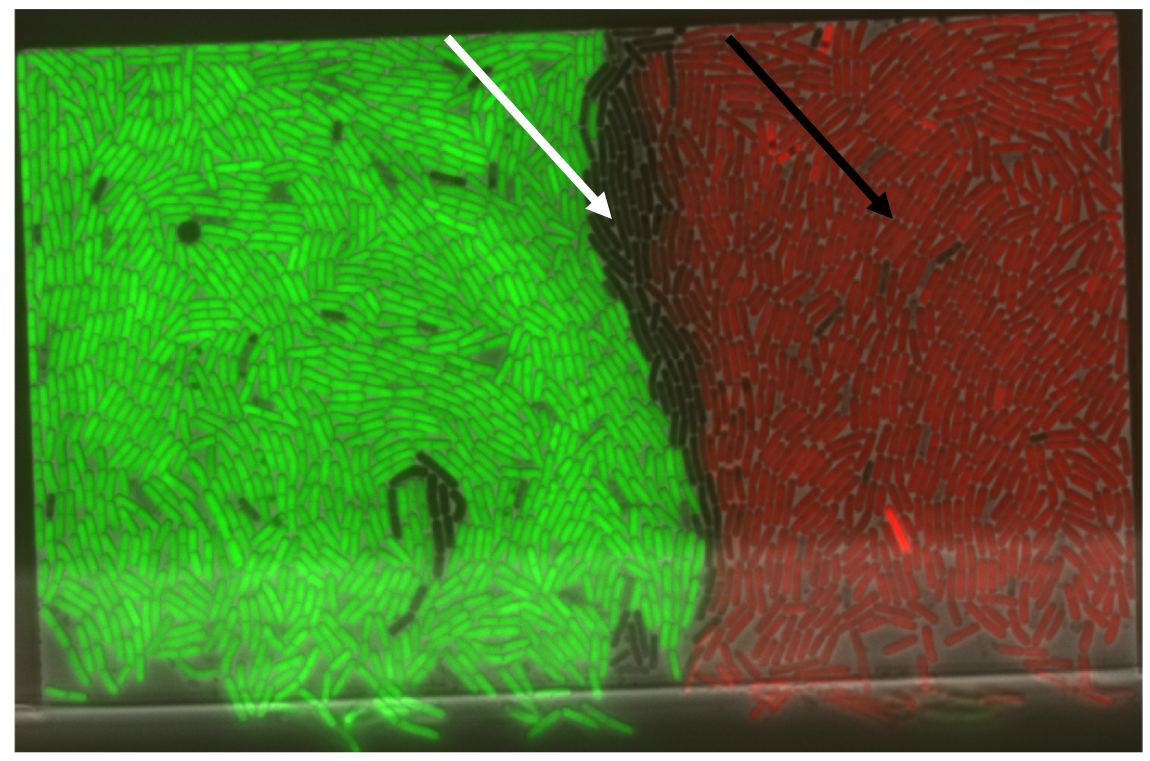
\includegraphics[width=\textwidth]{../figures/switchLikeReal.png}
        \caption{Microfluidics Chamber}
        \label{fig:mono_dec_real}
    \end{subfigure}
    \label{fig:mono_dec_comparison}
\end{figure}

% ============================================================================
% nonMONOTONIC  CIRCUIT
% ============================================================================
\section{Non-Monotonic Circuit}

\subsection{Circuit}

\begin{figure}[H]
    \centering
    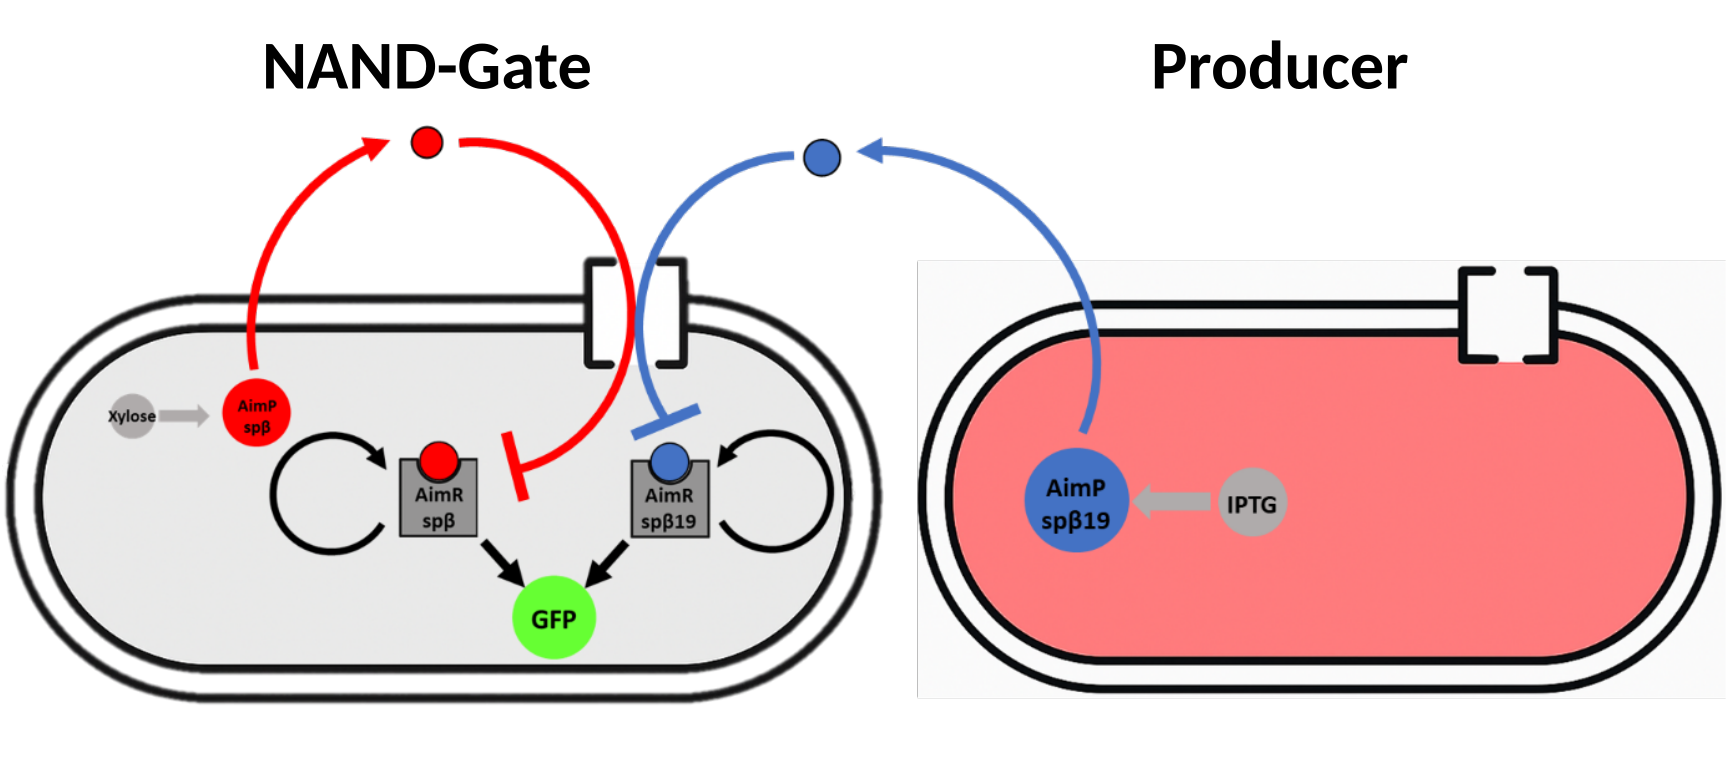
\includegraphics[width=0.8\textwidth]{../figures/nonMonDia.png}
    \label{fig:mono_dec_schematic}
\end{figure}



Intracellular AimP ($P_i$), AimP sp$\beta$19 ($P^*_i$), AimR ($R_i$), and AimR sp$\beta$19 ($R^*_i$) for a NAND-Gate bacteria $i$ at a location $r_i$:
\begin{align*}
\frac{\partial P_i}{\partial t} =& K_{in} P(r_i)^{ext} - K_{on} P_i R_i - \beta P_i\\
\frac{\partial P^*_i}{\partial t} =& K_{in} P^*(r_i)^{ext} - K_{on} P^*_i R^*_i - \beta P^*_i\\
\frac{\partial R_i}{\partial t} =& K_b + K_{syn}  \frac{R_i^n}{K_r^n + R_i^n} - K_{on} P_i R_i - \alpha R_i\\
\frac{\partial R^*_i}{\partial t} =& K_b + K_{syn}  \frac{(R^*_i)^n}{K_r^n + (R^*_i)^n} - K_{on} P^*_i R^*_i - \alpha R^*_i
\end{align*}

\textbf{Extracellular AimP and AimP sp$\beta$19  concentration:}
\begin{align*}
\frac{\partial P(r)^{ext}}{\partial t} =& K_{out} \frac{x}{K_x + x}\sum_{j}^{N} \delta(r_j - r) - K_{in} \sum_{b}^{N} P(r_b)^{ext}\delta(r_b - r)+ D_p \cdot \nabla^2 P(r)^{ext}\\
\frac{\partial P^*(r)^{ext}}{\partial t} =& K_{out} \frac{I}{K_{I} + I} \sum_{o}^{N} \delta(r_o - r)  - K_{in} \sum_{b}^{N} P^*(r_b)^{ext}\delta(r_b - r)+ D_p \cdot \nabla^2 P^*(r)^{ext}
\end{align*}
 

Where $x$ is xylose, $I$ is IPTG, $n$ is the Hill coefficient, $o$ is a producer bacteria, and $j$ is a NAND-Gate bacteria.

\subsection{Simulation vs. Real-World Comparison}

\begin{figure}[H] 
    \centering
    \begin{subfigure}[b]{0.45\textwidth}
        \centering
        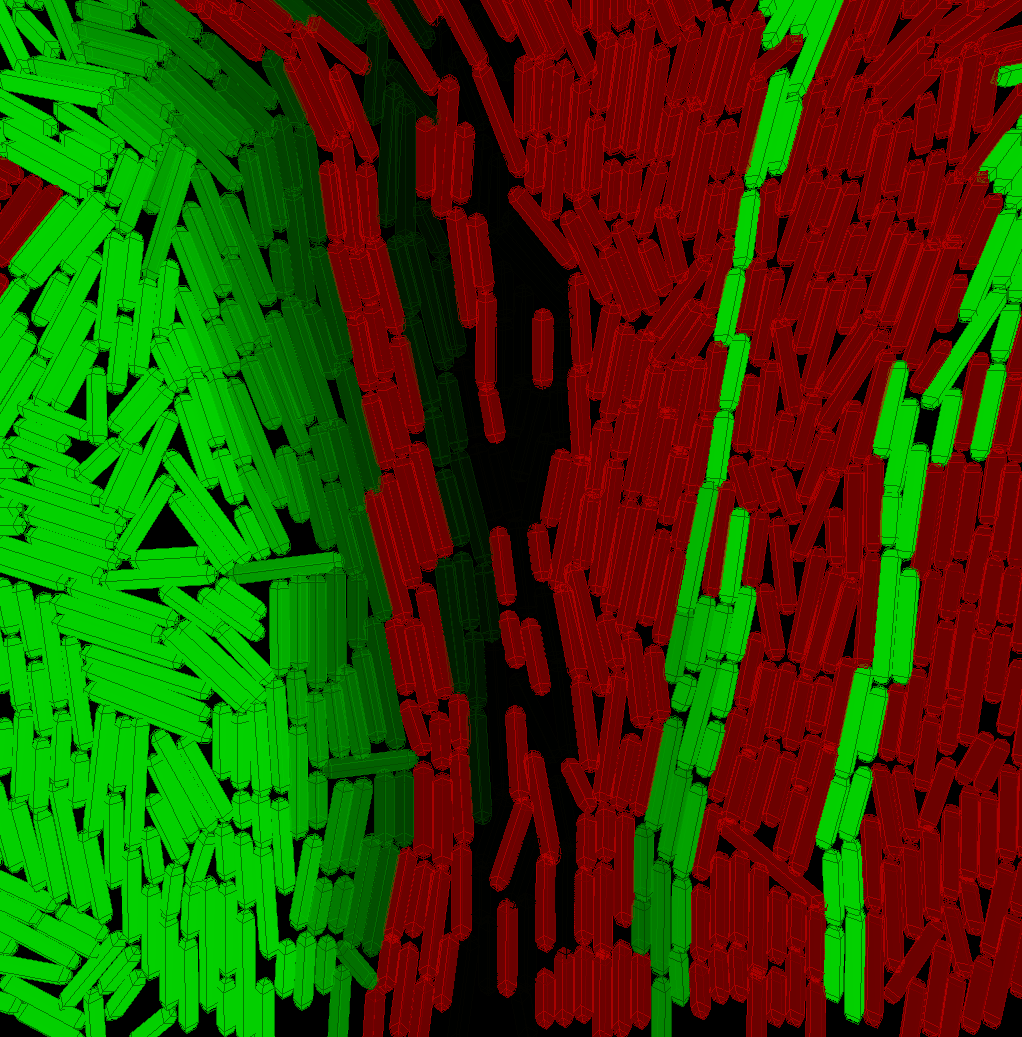
\includegraphics[width=\textwidth]{../figures/nonMono.png}
        \caption{Simulation Result}
        \label{fig:mono_dec_sim}
    \end{subfigure}
    \hfill
    \begin{subfigure}[b]{0.45\textwidth} 
        \centering
        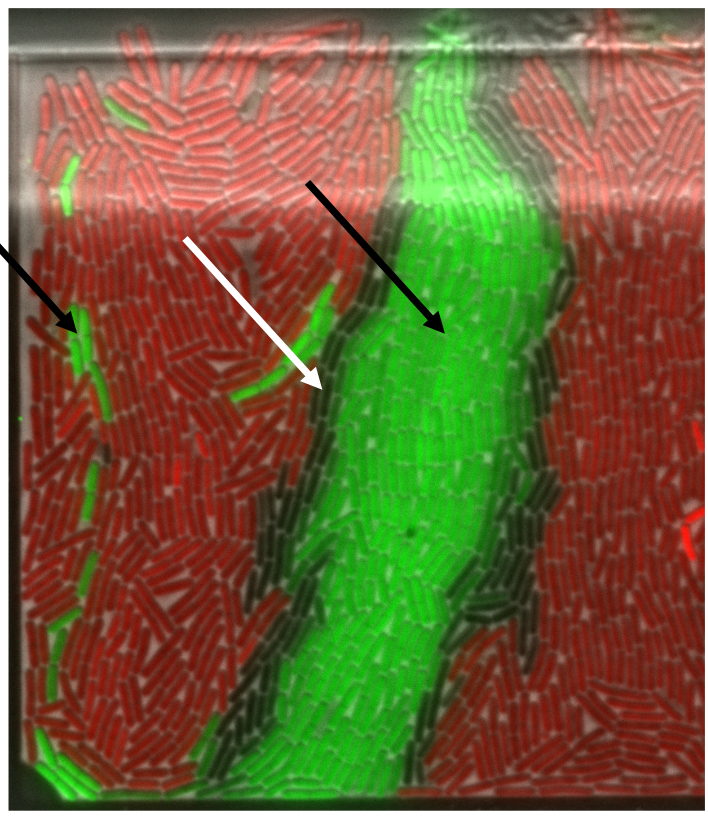
\includegraphics[width=\textwidth]{../figures/nonMonReal.png}
        \caption{Microfluidics Chamber}
        \label{fig:mono_dec_real}
    \end{subfigure}
    \label{fig:mono_dec_comparison} 
\end{figure}

\end{document}
